% !TeX root = ../main.tex

\chapter{LAMMPS 的性能测试和分析}
通过前两章内容的描述,我们给出了在申威众核平台上针对 eFF 势函数在计算,访存,通信等多个方面的并行和优化方案。本章会继续在对具体算例的实验中对这些优化方案进行测试工作,实验会在神威·太湖之光上以优化策略的性能对比和在大规模节点上以扩展性的形式呈现,并且这里对每一步优化后的结果和误差都进行了正确性验证。本章分为三节,第一节给出在神威·太湖之光与通用平台上的硬件对比,以及在测试时使用到的不同类型和规模的算例介绍。第二节是针对不同优化策略和组合对于提升整体计算性能效果的测试,进而分析对于LAMMPS 计算下访存,通信等应用特征。最后通过扩展性测试给出优化策略在大规模节点下的性能展示。下面给出实验中用到的不同优化方案及其组合:

\section{实验配置及算例介绍}
本文主要优化策略均在申威众核平台上进行,为对比不同平台间的性能差异,除在神威·太湖之光上进行测试之外,还进行了通用 X86 处理器平台上的性能分析对比实验,平台具体参数如下:

\begin{table}[]
     \centering
  \caption{SW26010 environment configuration}
\begin{tabular}{lll}
\hline
       & SW26010处理器  & Intel Xeon CPU E5-2660 \\ \hline
主频(主核) & 1.45        & 2.2                    \\
主频(从核) & 1.45        & /                      \\
内存     & 8           & 8                      \\
页表大小   & 8           & 4                      \\
编译器    & mpicc/sw5cc & mpicc                  \\ \hline
\end{tabular}
\end{table}

针对 LAMMPS 中 eFF 势函数的计算,这里选取了冲击波诱导电离界面模拟。模拟体系中共包含三类粒子,氢原子核,锂原子核和电子。时间步选取为0.005fs,系综为 NVE,截断半径根据当前粒子类型动态决定,采用圆柱模型模拟,xy 方向为固定边界条件,z 方向采用周期性边界条件,初始温度为300,测试单位以每时间步耗时作为性能指标。

\section{不同优化策略的加速效果}
当前测试算例规模选取了118000 个粒子,其中共由两类原子核和电子构成,迭代总步数为 5000 步,下面对每个时间步的计算时间进行测试,不同优化策略的性能对比如下图所示:

 \begin{figure}[h]
  \centering
  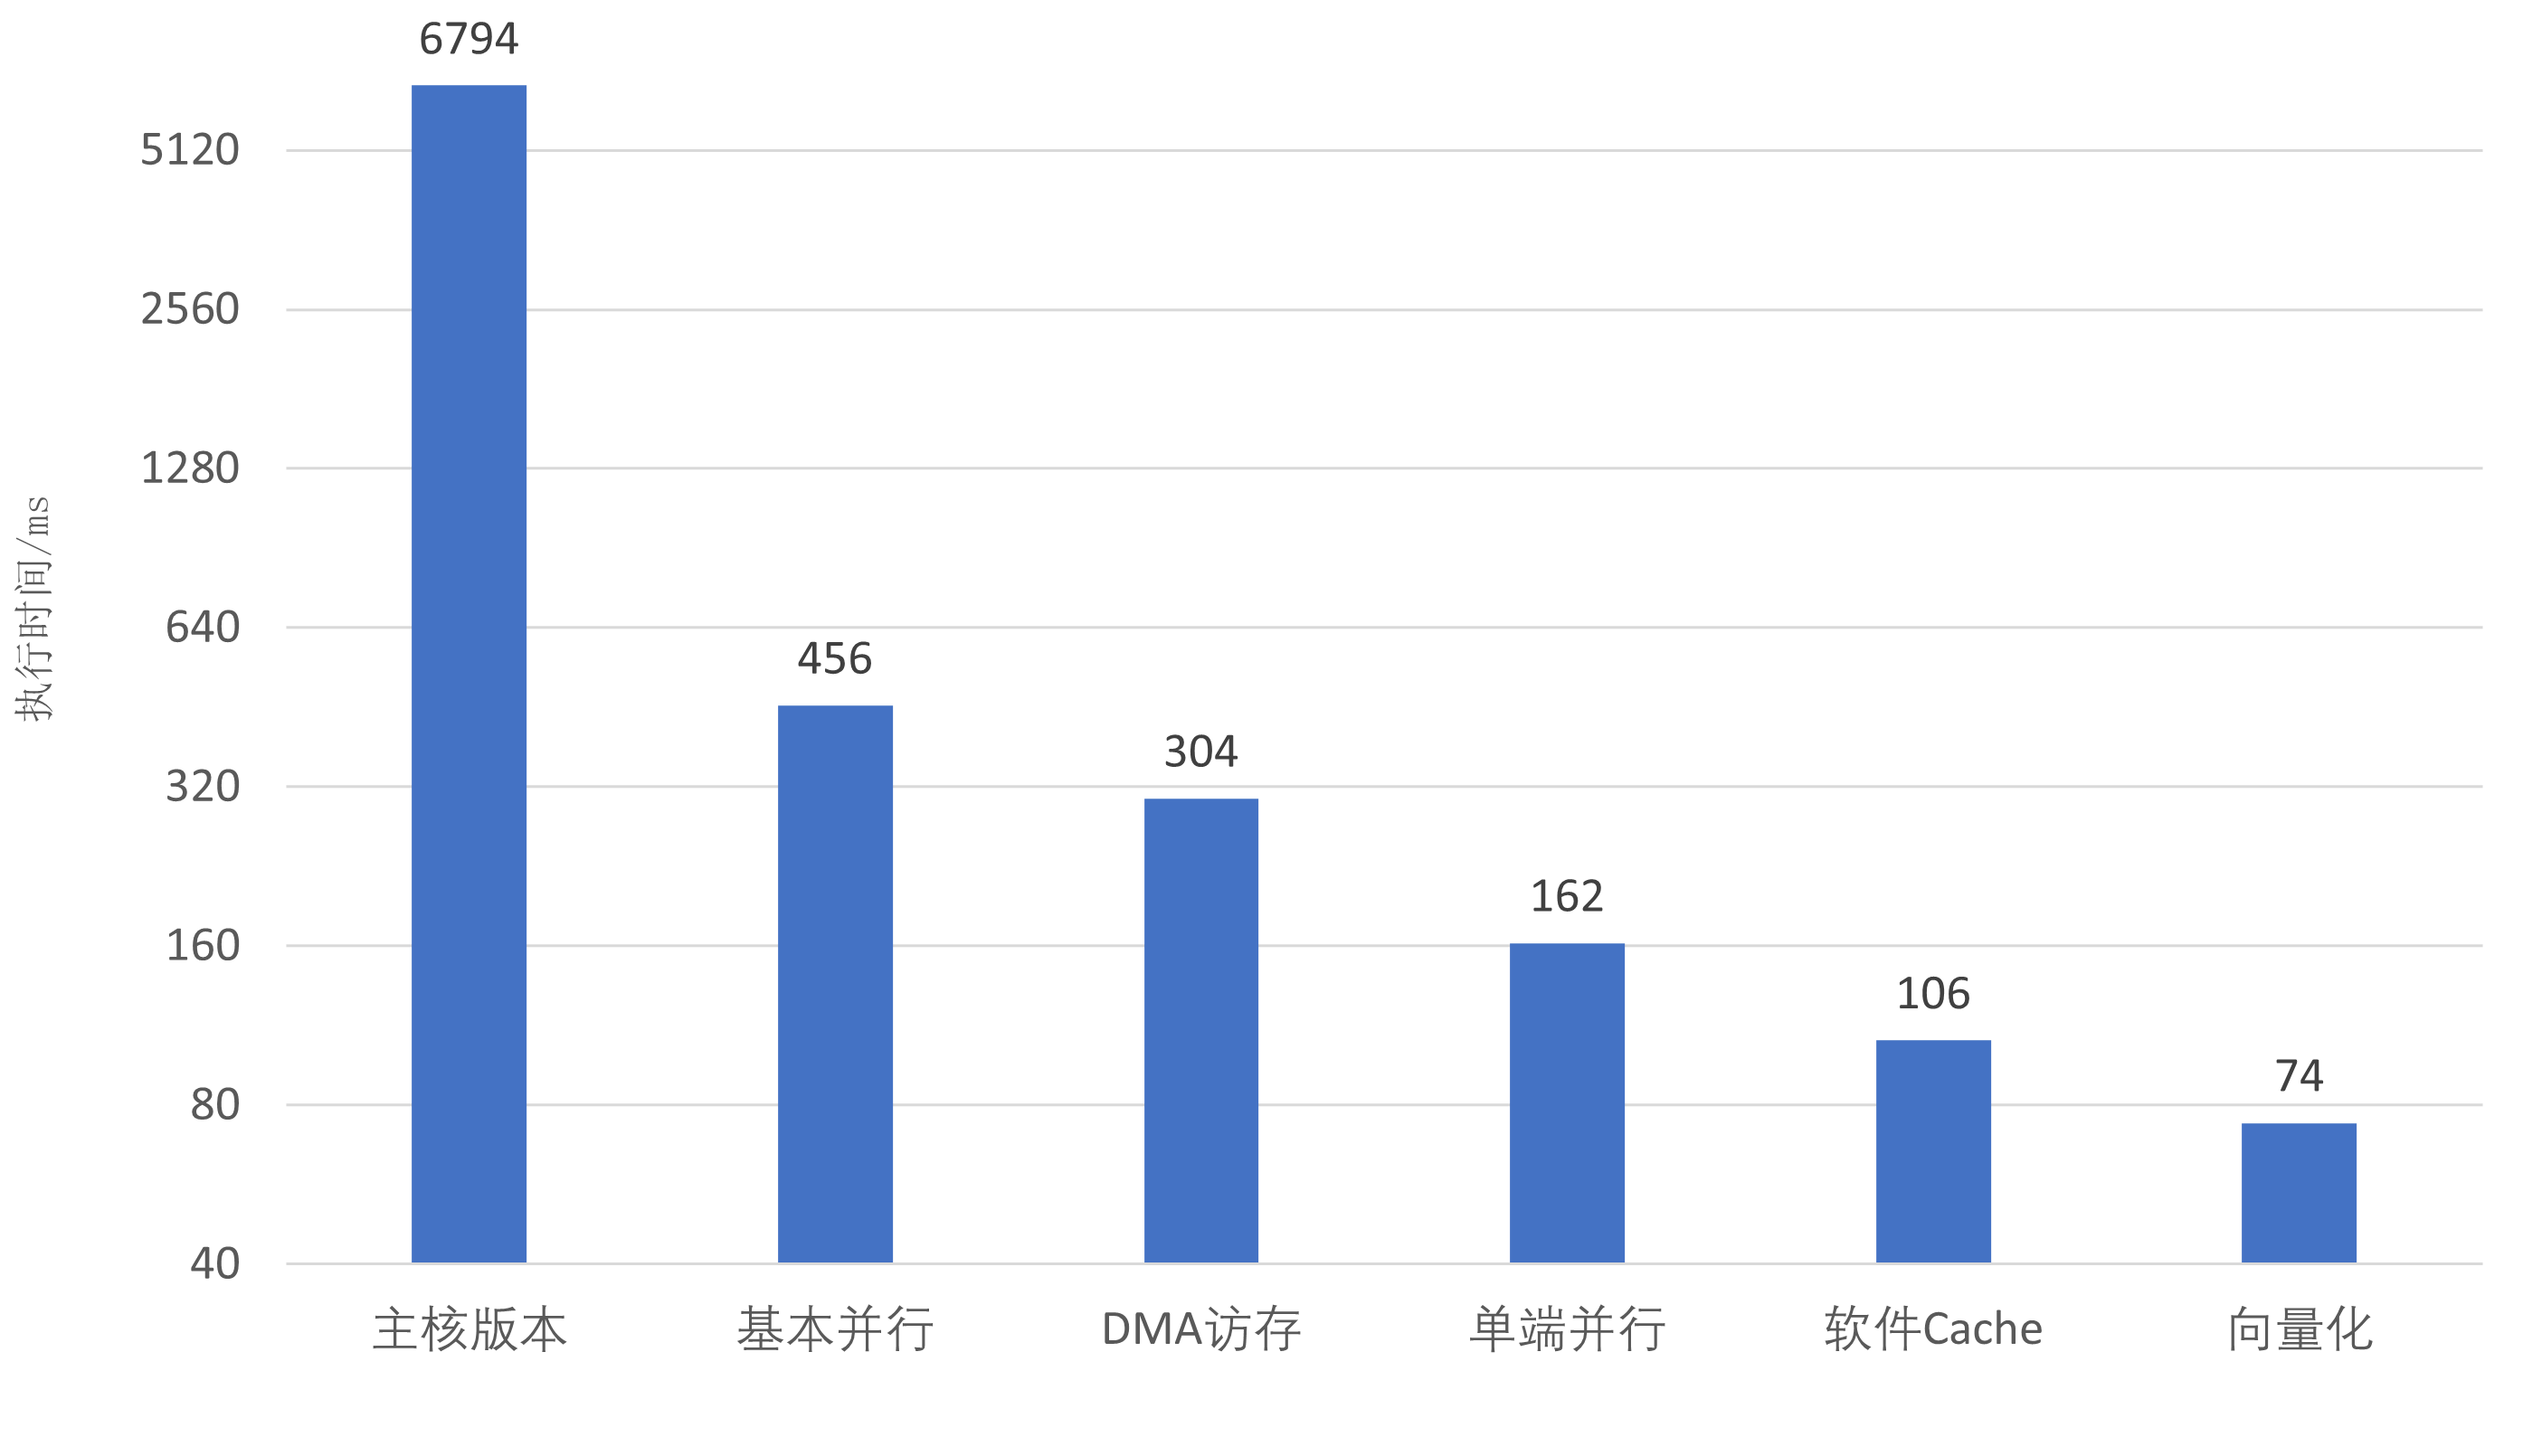
\includegraphics[width=0.8\textwidth]{opt_exp.png}
  \caption{不同优化配置下LAMMPS 的执行时间}
\end{figure}

通过性能测试的结果我们可以看出,在只通过主核进行计算时,每个时间步迭代的时间达到了 6794ms,这是由于主核在计算过程中不仅要完成热点函数的计算部分,还有进行I/O 操作,任务分发等工作,并且主核内的计算单元相对不足,导致性能结果不佳。在采用内层循环并行方案后,可以看到计算耗时有个明显地下降,这里是因为从核阵列的加入,使得邻居粒子的计算能够均匀分配到每个从核上,热点函数计算速度大幅提升,与此同时又引入了从核访存的开销问题。这里我们可以看出在使用 64 个从核同时进行计算后,整体的时间并没有表现出预取等比例地下降,因为仅仅引入计算的并行策略,增加访存开销的同时,也无法合理利用从核访存带宽。单次的 gld/gst 请求就会占用数百个时钟周期,此时访存开销成为了阻碍性能发挥的关键。在进行DMA 访存优化时,我们将原本需要多次访问才获取到的大块连续数据利用 DMA 方法采用单次的读写操作即可一次完成。这不仅降低了从核阵列内由于计算密度带来的频繁访存,也缓解了整体访存带宽的压力,至此的优化方法仅是对通用策略上的分析,还没有利用应用的具体特征进行深度优化。接下来通过更新并行策略来继续提高访存性能,采用单端更新的方法通过牺牲部分计算量,来换取更高的访存性能和并行度,这种方法支持大规模计算体系,扩展性也更强。尤其对于计算量较小,粒子排布较为稀疏的情况下发挥更好,从实验结果可以看出,针对 eFF 计算这种两体势来说,性能提升也较为明显,缺点就是固然会提升一定的计算量,但这种计算与访存性能之间的平衡却值得一试。为了进一步利用邻居粒子的局部性特征,通过在LDM 上开辟额外空间实现软件Cache 的做法也命中了超过百分之六十的粒子数据,访存频率和平均访存时间大幅减少,但软件Cache 实现的复杂性使其在性能提升方面不能与通用 CPU 上的多级 Cache 设计相比。至此,已经完成了对访存性能全部优化策略的分析。由于访存开销在整个体系计算中的比例降低和在单端更新并行方法中引入了更多的计算量,导致计算部分在势函数计算中占据了更大的部分。这里继续通过向量化指令和向量混洗操作,解决了离散粒子数据的读取和分支计算问题,使计算时间大幅降低。

除了对不同实验配置和优化方案给出量化的性能结果外,这里也展示了在采用多个并行和优化方法的过程中,每种优化方案单独的性能提升在总性能优化中的地位,这同时也可以看出 eFF 势函数计算中对于不同应用特征每种策略产生的优化效果,也可以对访存,计算,通信等在申威平台上常见的处理问题进行总结。这里多种方案以不同的顺序进行累加测试后优化幅度可能会略有差异,例如采用单端更新方法会提升计算量,从而提高向量化的优化比例。

进行神威·太湖之光上各优化策略的性能测试后,这里也设计了不同优化阶段与通过 X86 平台上 eFF 势计算性能的对比实验。其中通用平台采用的计算核心数量与从核进行数量保持一致,采用相同的算例进行测试。可以看出通用处理器的性能与进行从核并行与访存优化后的性能相接近。这一方面是因为通用处理器的访存带宽要高于 SW26010 处理器,另一方面是多层 Cache 的设计使得数据重用性有着大幅的改善,访存频率也有着显著的降低。在从核采用软件Cache和向量化方法之后,访存和计算效率有了很大改善,性能也随之进行了反超。

 \begin{figure}[h]
  \centering
  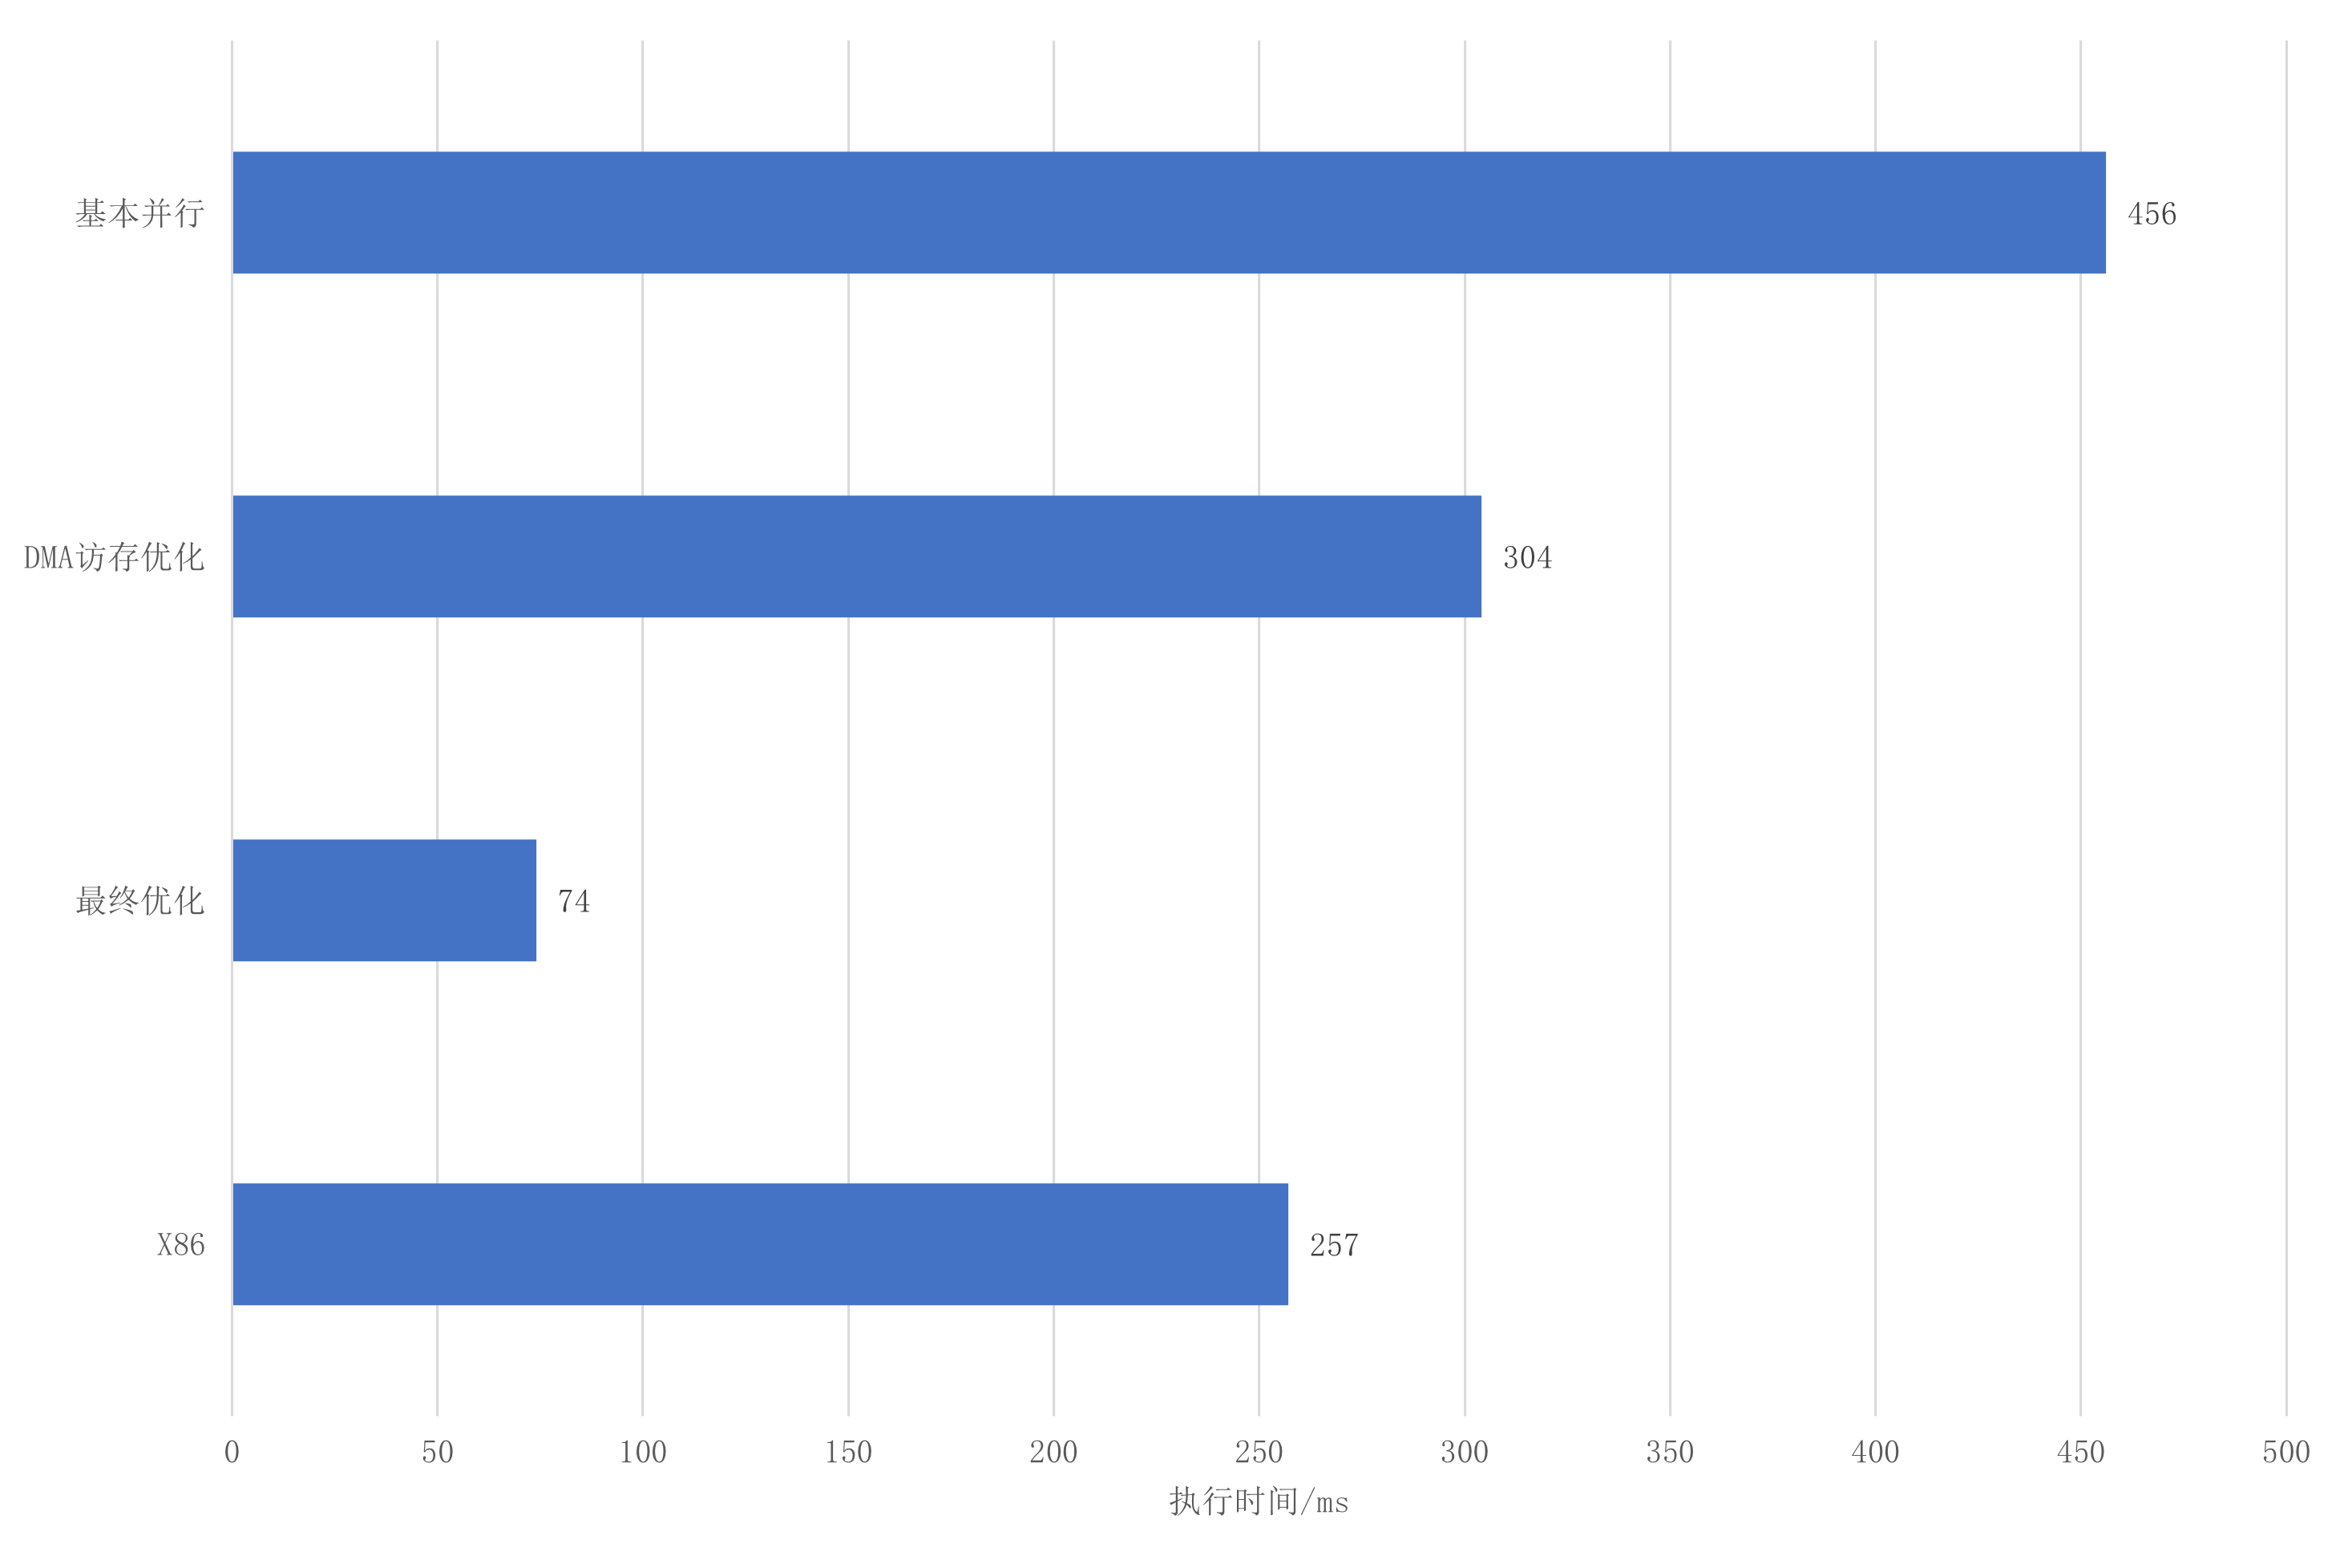
\includegraphics[width=0.8\textwidth]{platf_exp.png}
  \caption{申威平台LAMMPS 性能与通用平台比较}
\end{figure}

为了保证在程序算法在进行并行优化后,结果不会产生影响正确性的误差,这里还设计了程序正确性上的比对。通过比较在申威平台与通用平台上的计算结果,来保证结果的一致性,这里使用与上述相同的计算算例,选择了50000 个时间步作为模拟时长,在模拟过程中比较温度的变化来验证结果正确性。采用全部优化策略后的方案与通用平台上的计算温度的变化如图所示,从图中可以看出,在整个模拟进行的过程中,通用平台与优化后算法在相同算例下的温度变化基本一致。

\section{扩展性测试}
在分析完每一种优化方案对应用性能的提升幅度后,进行神威·太湖之光平台上 eFF 势函数计算的扩展性测试,进而总结出这部分计算在大规模模拟时的计算性能。这里的扩展性实验共分为两部分,强扩展性测试和弱扩展性测试,其中强扩展性时再总计算规模固定时,随着计算处理单元的递增,程序性能表现出来的趋势。弱扩展性是指在每个处理单元分配相同的任务量,随着计算规模和处理器数量等比例增长,性能表现出来的趋势。这里给出扩展效率的表达公式:

\begin{equation}
  U_N=\frac{T_a}{T_N}\cdot \frac{a}{N}
\end{equation}

其中𝑈𝑁 表示在处理核心数量在a 和N 时的程序扩展性,T 表示程序运行的耗时。

首先进行强扩展性测试,在这部分测试中,选取 980 万的粒子规模进行计算,进程数从 4 个开始逐步递增,最大计算进程数达到 65536 个。在此基础上,先通过设置理想情况下的性能扩展性,也就是性能性能随着进程数同比例增加,再与当前规模下的实际性能进行对比,得出扩展效率。从结果中可以观察到,随着计算进程的增多,LAMMPS 的实际性能与理想性能之间的偏差逐渐增大。这是因为总计算规模不变的情况下,参与计算的进程数量不断提高,导致每个进程负责的粒子计算不断变少,在进程数达到最大的时候,每个进程只分配了不到200 个粒子,此时在进程反而边界粒子占据了多数,使得扩展效率只有不到百分之六十。

 \begin{figure}[h]
  \centering
  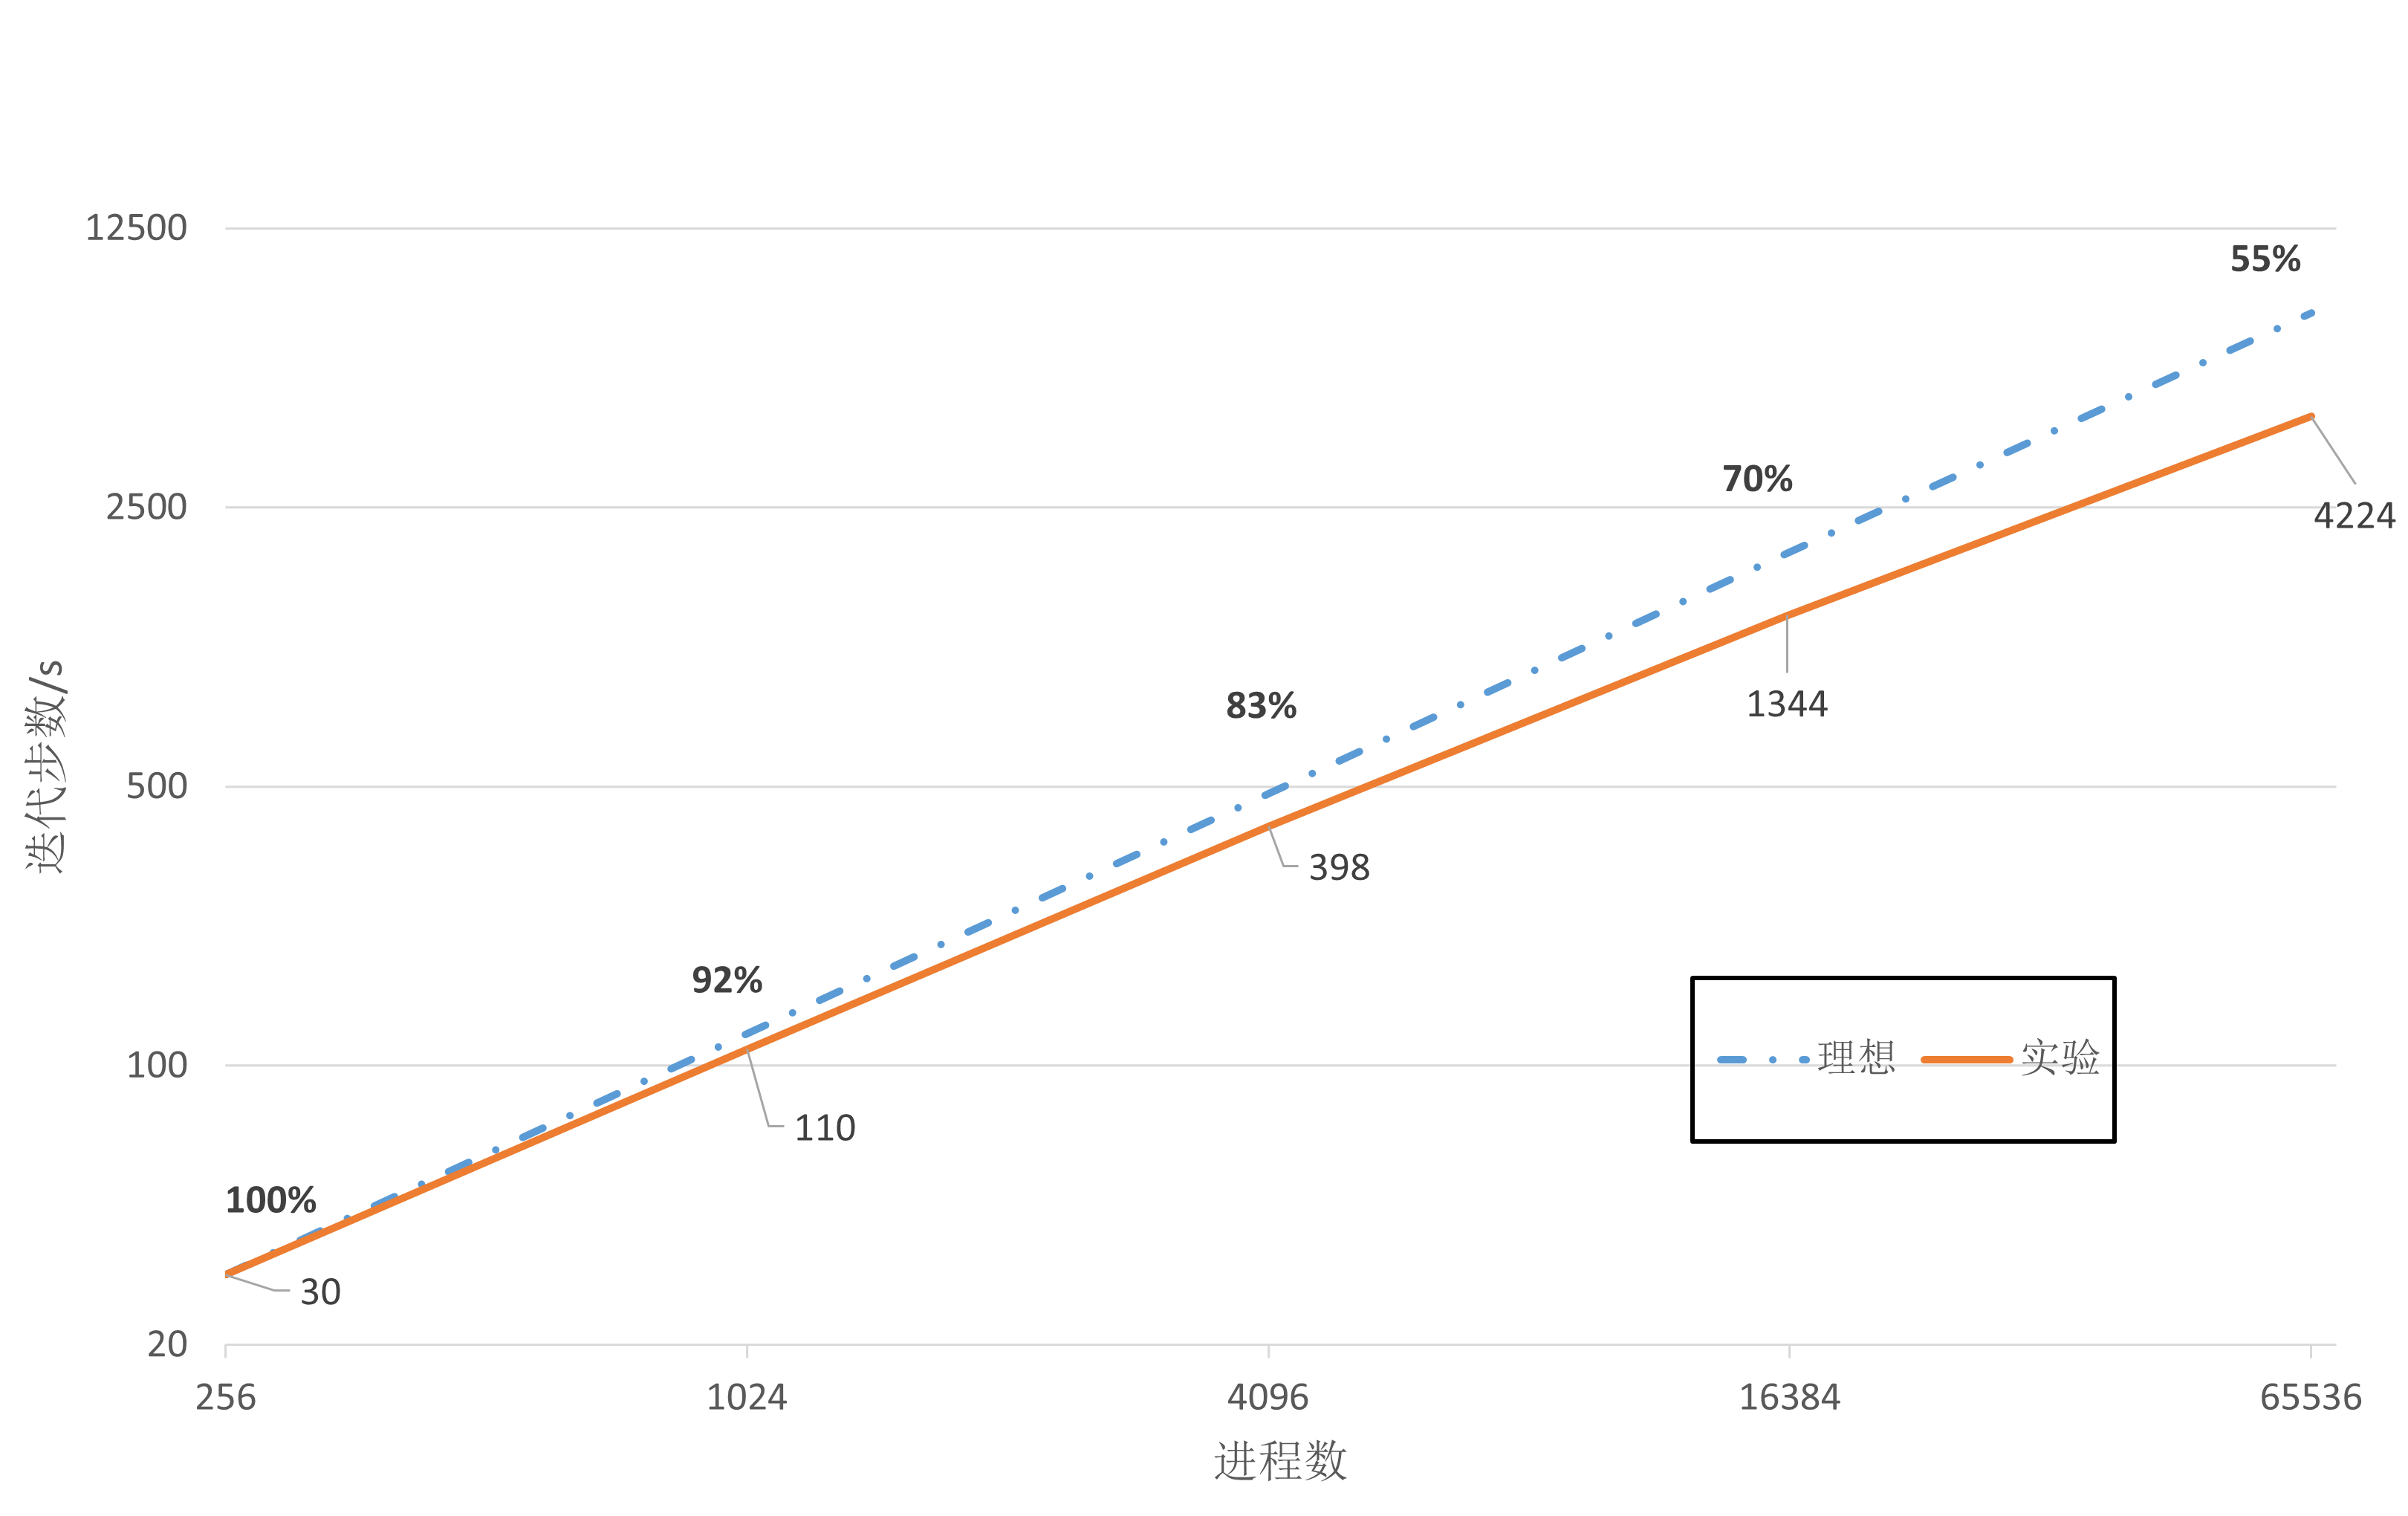
\includegraphics[width=0.8\textwidth]{s_scale.png}
  \caption{LAMMPS 强扩展性测试}
\end{figure}

 接下来进行弱扩展性测试,在这部分测试中,每个进程保持一定的粒子规模,算例总的粒子数随着进程数量等比例地增加,最大进程数同样达到65536 个。从结果中可以观察到,与强扩展性测试不同的是,整体扩展性不会随着进程数的增大而有着明显的变化,这是因为在每个进程中的粒子数量基本相同,进程在时间步之间的计算量不会发生太大的变化,所以弱扩展性的结果表现稳定的状态。

  \begin{figure}[h]
  \centering
  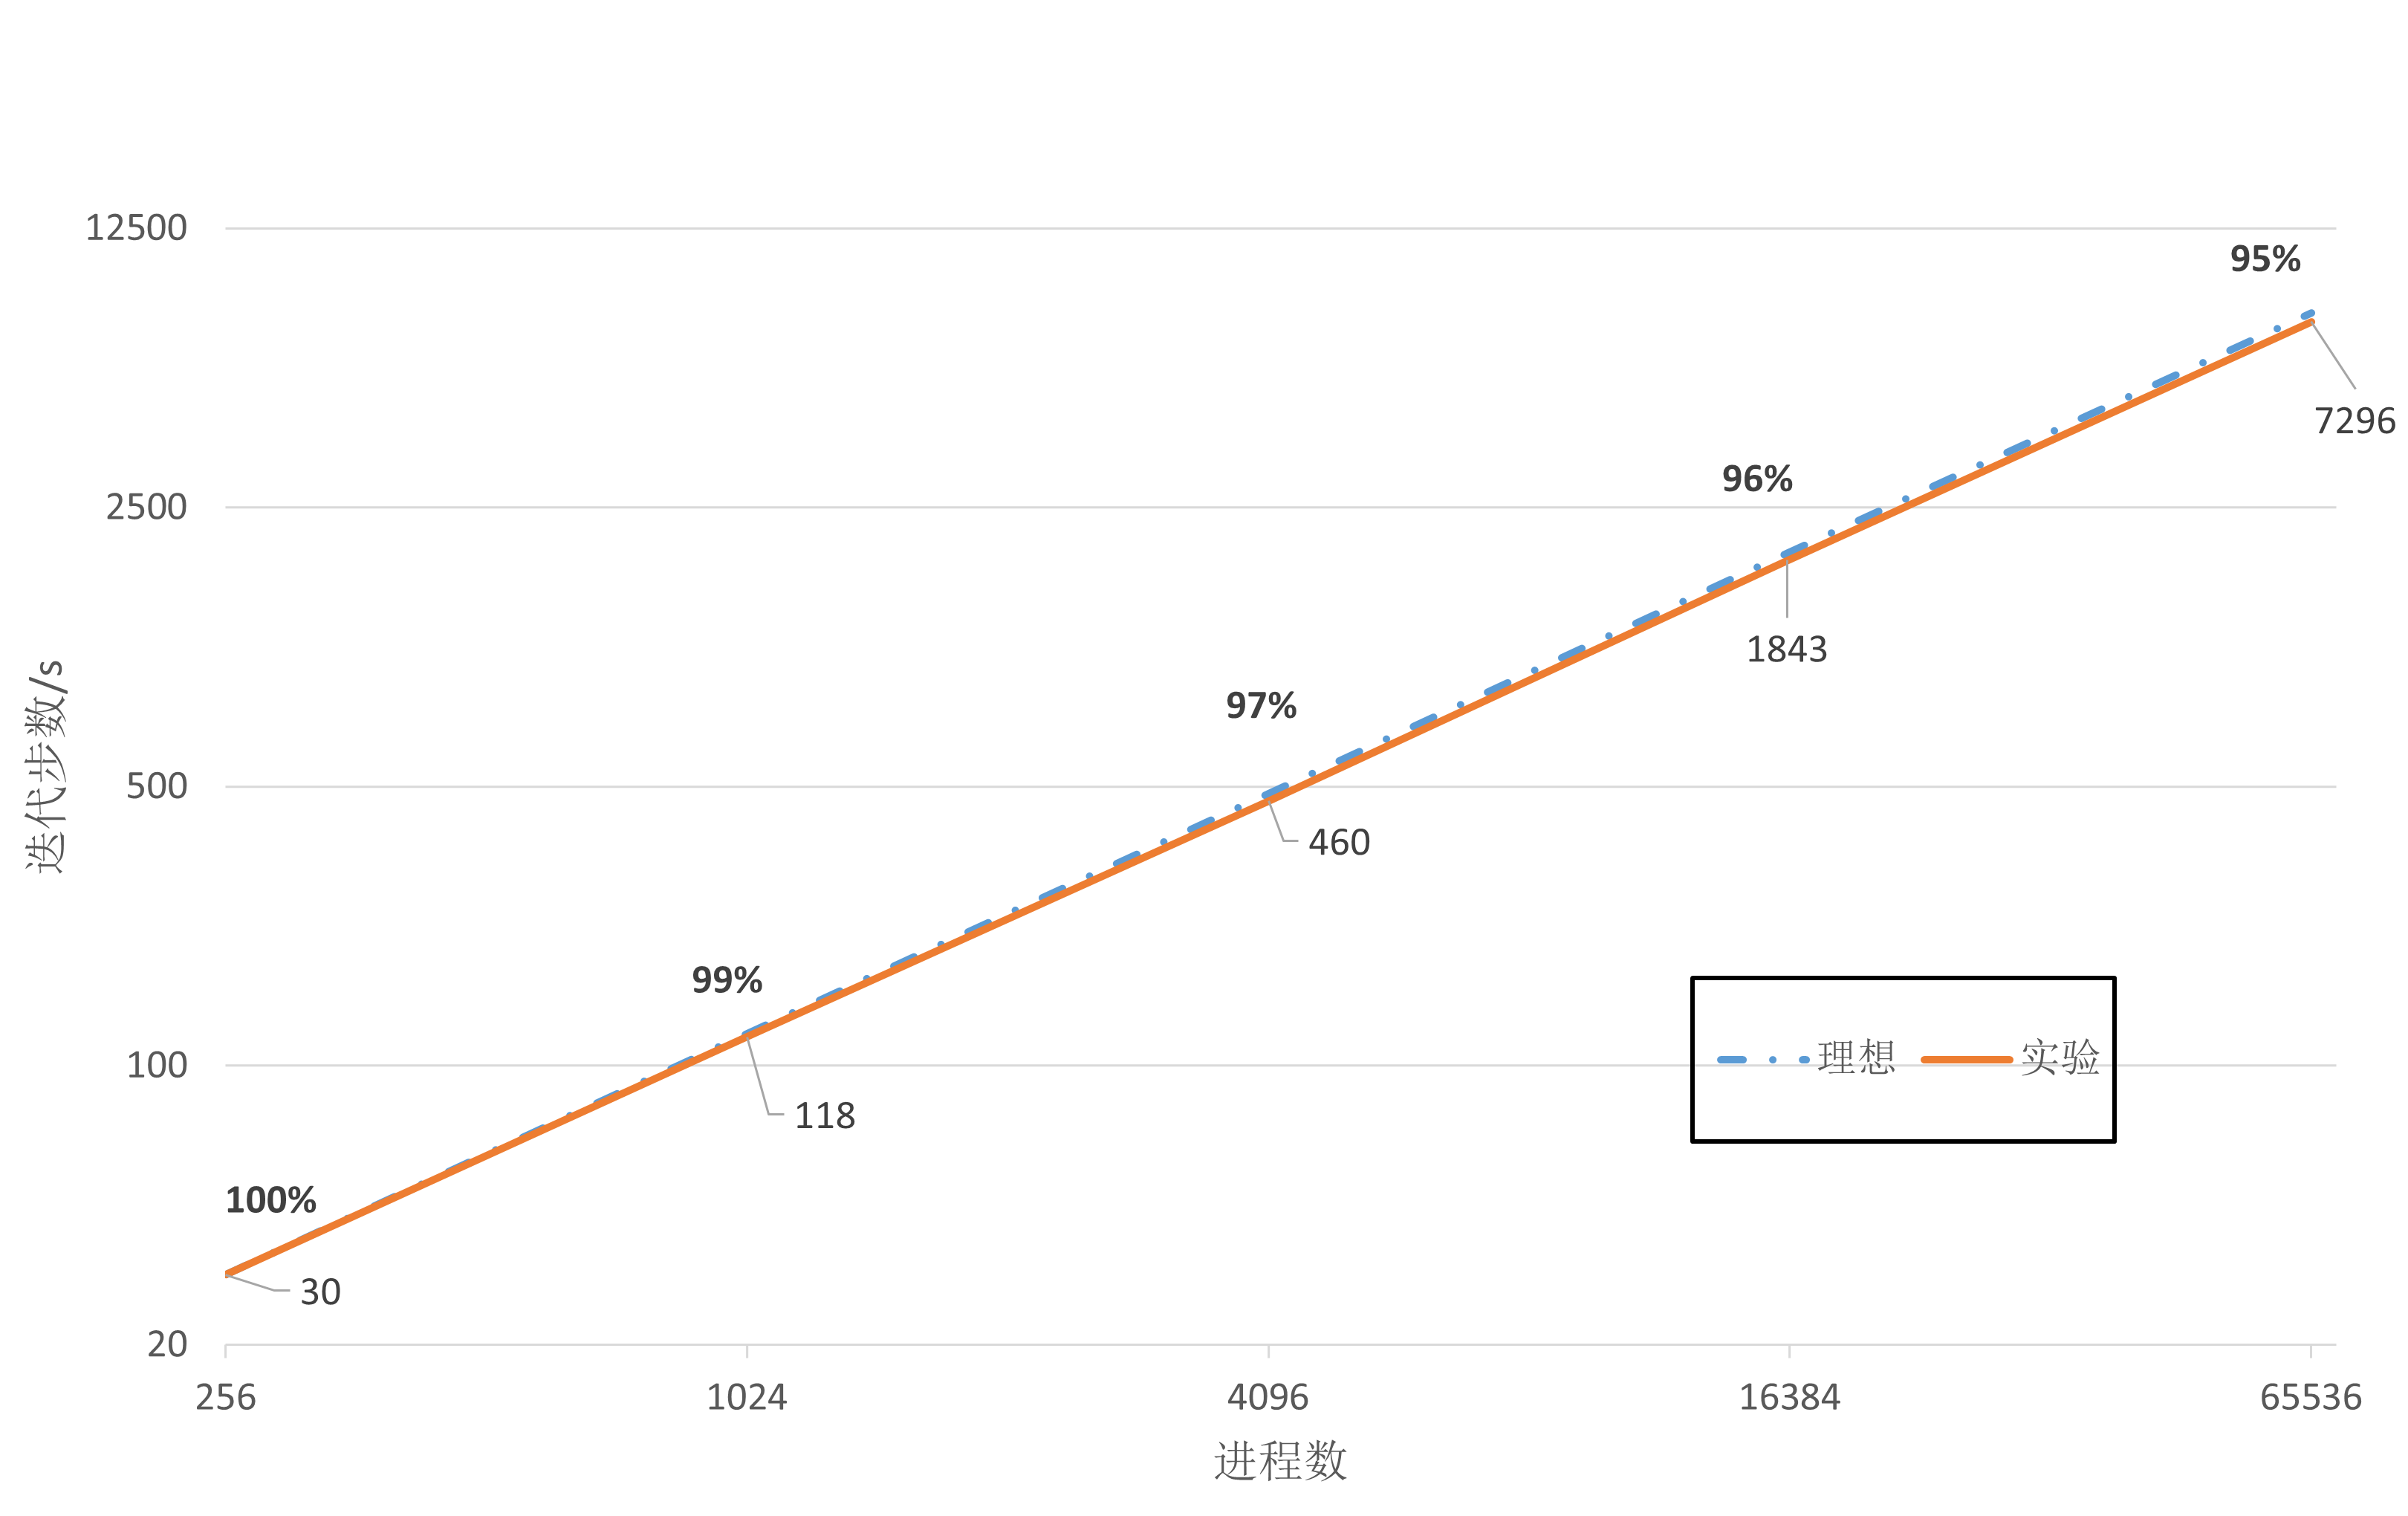
\includegraphics[width=0.8\textwidth]{w_scale.png}
  \caption{LAMMPS 弱扩展性测试}
\end{figure}

\section{本章小结}
本章展示出文章中提出优化策略的测试工作,涉及多种并行方案,访存,通信和计算的多种策略的性能分析,也给出了大规模计算中LAMMPS 的扩展性测试。首先测试了不同优化方案对于 eFF 势函数计算的性能提升情况,并通过方案间的具体加速比,分析了不同方案对总优化的贡献分配。测试表明在经过不同方案的性能加速后,并行版本的 eFF 计算相比于主核版本产生了 91 倍的性能提升,并且对于通用平台处理器,也有着不小的性能领先。在性能优化的同时验证了计算的正确性,使 X86 平台上的结果误差保持在可接受的范围内。接下来给出eFF 计算在神威·太湖之光上的扩展性测试,通过调整实际算例的规模,将计算进行增至 65536 个,分别得到了 55\% 的强扩展性和 88\% 的弱扩展性。
